% Options for packages loaded elsewhere
\PassOptionsToPackage{unicode}{hyperref}
\PassOptionsToPackage{hyphens}{url}
%
\documentclass[
  man]{apa7}
\usepackage{amsmath,amssymb}
\usepackage{iftex}
\ifPDFTeX
  \usepackage[T1]{fontenc}
  \usepackage[utf8]{inputenc}
  \usepackage{textcomp} % provide euro and other symbols
\else % if luatex or xetex
  \usepackage{unicode-math} % this also loads fontspec
  \defaultfontfeatures{Scale=MatchLowercase}
  \defaultfontfeatures[\rmfamily]{Ligatures=TeX,Scale=1}
\fi
\usepackage{lmodern}
\ifPDFTeX\else
  % xetex/luatex font selection
\fi
% Use upquote if available, for straight quotes in verbatim environments
\IfFileExists{upquote.sty}{\usepackage{upquote}}{}
\IfFileExists{microtype.sty}{% use microtype if available
  \usepackage[]{microtype}
  \UseMicrotypeSet[protrusion]{basicmath} % disable protrusion for tt fonts
}{}
\makeatletter
\@ifundefined{KOMAClassName}{% if non-KOMA class
  \IfFileExists{parskip.sty}{%
    \usepackage{parskip}
  }{% else
    \setlength{\parindent}{0pt}
    \setlength{\parskip}{6pt plus 2pt minus 1pt}}
}{% if KOMA class
  \KOMAoptions{parskip=half}}
\makeatother
\usepackage{xcolor}
\usepackage{graphicx}
\makeatletter
\def\maxwidth{\ifdim\Gin@nat@width>\linewidth\linewidth\else\Gin@nat@width\fi}
\def\maxheight{\ifdim\Gin@nat@height>\textheight\textheight\else\Gin@nat@height\fi}
\makeatother
% Scale images if necessary, so that they will not overflow the page
% margins by default, and it is still possible to overwrite the defaults
% using explicit options in \includegraphics[width, height, ...]{}
\setkeys{Gin}{width=\maxwidth,height=\maxheight,keepaspectratio}
% Set default figure placement to htbp
\makeatletter
\def\fps@figure{htbp}
\makeatother
\setlength{\emergencystretch}{3em} % prevent overfull lines
\providecommand{\tightlist}{%
  \setlength{\itemsep}{0pt}\setlength{\parskip}{0pt}}
\setcounter{secnumdepth}{-\maxdimen} % remove section numbering
% Make \paragraph and \subparagraph free-standing
\ifx\paragraph\undefined\else
  \let\oldparagraph\paragraph
  \renewcommand{\paragraph}[1]{\oldparagraph{#1}\mbox{}}
\fi
\ifx\subparagraph\undefined\else
  \let\oldsubparagraph\subparagraph
  \renewcommand{\subparagraph}[1]{\oldsubparagraph{#1}\mbox{}}
\fi
\newlength{\cslhangindent}
\setlength{\cslhangindent}{1.5em}
\newlength{\csllabelwidth}
\setlength{\csllabelwidth}{3em}
\newlength{\cslentryspacingunit} % times entry-spacing
\setlength{\cslentryspacingunit}{\parskip}
\newenvironment{CSLReferences}[2] % #1 hanging-ident, #2 entry spacing
 {% don't indent paragraphs
  \setlength{\parindent}{0pt}
  % turn on hanging indent if param 1 is 1
  \ifodd #1
  \let\oldpar\par
  \def\par{\hangindent=\cslhangindent\oldpar}
  \fi
  % set entry spacing
  \setlength{\parskip}{#2\cslentryspacingunit}
 }%
 {}
\usepackage{calc}
\newcommand{\CSLBlock}[1]{#1\hfill\break}
\newcommand{\CSLLeftMargin}[1]{\parbox[t]{\csllabelwidth}{#1}}
\newcommand{\CSLRightInline}[1]{\parbox[t]{\linewidth - \csllabelwidth}{#1}\break}
\newcommand{\CSLIndent}[1]{\hspace{\cslhangindent}#1}
\ifLuaTeX
\usepackage[bidi=basic]{babel}
\else
\usepackage[bidi=default]{babel}
\fi
\babelprovide[main,import]{english}
% get rid of language-specific shorthands (see #6817):
\let\LanguageShortHands\languageshorthands
\def\languageshorthands#1{}
% Manuscript styling
\usepackage{upgreek}
\captionsetup{font=singlespacing,justification=justified}

% Table formatting
\usepackage{longtable}
\usepackage{lscape}
% \usepackage[counterclockwise]{rotating}   % Landscape page setup for large tables
\usepackage{multirow}		% Table styling
\usepackage{tabularx}		% Control Column width
\usepackage[flushleft]{threeparttable}	% Allows for three part tables with a specified notes section
\usepackage{threeparttablex}            % Lets threeparttable work with longtable

% Create new environments so endfloat can handle them
% \newenvironment{ltable}
%   {\begin{landscape}\centering\begin{threeparttable}}
%   {\end{threeparttable}\end{landscape}}
\newenvironment{lltable}{\begin{landscape}\centering\begin{ThreePartTable}}{\end{ThreePartTable}\end{landscape}}

% Enables adjusting longtable caption width to table width
% Solution found at http://golatex.de/longtable-mit-caption-so-breit-wie-die-tabelle-t15767.html
\makeatletter
\newcommand\LastLTentrywidth{1em}
\newlength\longtablewidth
\setlength{\longtablewidth}{1in}
\newcommand{\getlongtablewidth}{\begingroup \ifcsname LT@\roman{LT@tables}\endcsname \global\longtablewidth=0pt \renewcommand{\LT@entry}[2]{\global\advance\longtablewidth by ##2\relax\gdef\LastLTentrywidth{##2}}\@nameuse{LT@\roman{LT@tables}} \fi \endgroup}

% \setlength{\parindent}{0.5in}
% \setlength{\parskip}{0pt plus 0pt minus 0pt}

% Overwrite redefinition of paragraph and subparagraph by the default LaTeX template
% See https://github.com/crsh/papaja/issues/292
\makeatletter
\renewcommand{\paragraph}{\@startsection{paragraph}{4}{\parindent}%
  {0\baselineskip \@plus 0.2ex \@minus 0.2ex}%
  {-1em}%
  {\normalfont\normalsize\bfseries\itshape\typesectitle}}

\renewcommand{\subparagraph}[1]{\@startsection{subparagraph}{5}{1em}%
  {0\baselineskip \@plus 0.2ex \@minus 0.2ex}%
  {-\z@\relax}%
  {\normalfont\normalsize\itshape\hspace{\parindent}{#1}\textit{\addperi}}{\relax}}
\makeatother

\makeatletter
\usepackage{etoolbox}
\patchcmd{\maketitle}
  {\section{\normalfont\normalsize\abstractname}}
  {\section*{\normalfont\normalsize\abstractname}}
  {}{\typeout{Failed to patch abstract.}}
\patchcmd{\maketitle}
  {\section{\protect\normalfont{\@title}}}
  {\section*{\protect\normalfont{\@title}}}
  {}{\typeout{Failed to patch title.}}
\makeatother

\usepackage{xpatch}
\makeatletter
\xapptocmd\appendix
  {\xapptocmd\section
    {\addcontentsline{toc}{section}{\appendixname\ifoneappendix\else~\theappendix\fi\\: #1}}
    {}{\InnerPatchFailed}%
  }
{}{\PatchFailed}
\keywords{keywords\newline\indent Word count: X}
\DeclareDelayedFloatFlavor{ThreePartTable}{table}
\DeclareDelayedFloatFlavor{lltable}{table}
\DeclareDelayedFloatFlavor*{longtable}{table}
\makeatletter
\renewcommand{\efloat@iwrite}[1]{\immediate\expandafter\protected@write\csname efloat@post#1\endcsname{}}
\makeatother
\usepackage{lineno}

\linenumbers
\usepackage{csquotes}
\makeatletter
\renewcommand{\paragraph}{\@startsection{paragraph}{4}{\parindent}%
  {0\baselineskip \@plus 0.2ex \@minus 0.2ex}%
  {-1em}%
  {\normalfont\normalsize\bfseries\typesectitle}}

\renewcommand{\subparagraph}[1]{\@startsection{subparagraph}{5}{1em}%
  {0\baselineskip \@plus 0.2ex \@minus 0.2ex}%
  {-\z@\relax}%
  {\normalfont\normalsize\bfseries\itshape\hspace{\parindent}{#1}\textit{\addperi}}{\relax}}
\makeatother

\ifLuaTeX
  \usepackage{selnolig}  % disable illegal ligatures
\fi
\IfFileExists{bookmark.sty}{\usepackage{bookmark}}{\usepackage{hyperref}}
\IfFileExists{xurl.sty}{\usepackage{xurl}}{} % add URL line breaks if available
\urlstyle{same}
\hypersetup{
  pdftitle={The title},
  pdfauthor={First Author1 \& Ernst-August Doelle1,2},
  pdflang={en-EN},
  pdfkeywords={keywords},
  hidelinks,
  pdfcreator={LaTeX via pandoc}}

\title{The title}
\author{First Author\textsuperscript{1} \& Ernst-August Doelle\textsuperscript{1,2}}
\date{}


\shorttitle{Title}

\authornote{

Add complete departmental affiliations for each author here. Each new line herein must be indented, like this line.

Enter author note here.

The authors made the following contributions. First Author: Conceptualization, Writing - Original Draft Preparation, Writing - Review \& Editing; Ernst-August Doelle: Writing - Review \& Editing, Supervision.

Correspondence concerning this article should be addressed to First Author, Postal address. E-mail: \href{mailto:my@email.com}{\nolinkurl{my@email.com}}

}

\affiliation{\vspace{0.5cm}\textsuperscript{1} Wilhelm-Wundt-University\\\textsuperscript{2} Konstanz Business School}

\abstract{%
One or two sentences providing a \textbf{basic introduction} to the field, comprehensible to a scientist in any discipline.
Two to three sentences of \textbf{more detailed background}, comprehensible to scientists in related disciplines.
One sentence clearly stating the \textbf{general problem} being addressed by this particular study.
One sentence summarizing the main result (with the words ``\textbf{here we show}'' or their equivalent).
Two or three sentences explaining what the \textbf{main result} reveals in direct comparison to what was thought to be the case previously, or how the main result adds to previous knowledge.
One or two sentences to put the results into a more \textbf{general context}.
Two or three sentences to provide a \textbf{broader perspective}, readily comprehensible to a scientist in any discipline.
}



\begin{document}
\maketitle

Psychological research involves the difficult task of assessing non-observable phenomena, such as depression or meaning in life, as a measurement proxy for analyzing hypotheses. Researchers develop surveys or instruments to estimate the underlying construction of interest (DeVellis \& Thorpe, 2022), which is then often validated with latent variable modeling (i.e., structural equation modeling; SEM) or item response theory (IRT, Byrne, 2001). Confirmatory factor analysis (CFA) is the most common choice for examining questionnaire's dimensionality, item-latent variable structure, and the overall model fit. Entire journals, such as \emph{Assessment,} are devoted to the publication of scale development and (re)-assessment across different group populations - a necessary avenue given that development information for many scales is not reported in other journal articles (Barry et al., 2014; Weidman et al., 2017). These manuscripts are crucial to interpretation of studies that use these measures and determining the usefulness of overall measured scores (Flake \& Fried, 2020).

Generalized measures are designed, in theory, to provide the same assessment for different populations (Meredith, 1993); however, there is growing interest in examining for differential responding across sub-populations based on potentially confounding variables. Measurement invariance (or equivalence) implies that the instrument provides the same latent variable measurement for all populations. Equality in measurement is desirable, as it allows for the same interpretation of latent variable scores across groups, as well as knowing that group differences are not attributable to differences in measurement. Non-invariance implies that individuals in separate populations interpret items differently (Cheung \& Rensvold, 2000; Dong \& Dumas, 2020; Liu et al., 2017; Wicherts et al., 2005), which may affect the overall latent variable score; thus, making it difficult to know if group differences are due to population differences or measurement. Being unaware of non-invariance in measures could lead to incorrect interpretations of group differences (Van De Schoot et al., 2015), and these results could potentially explain the replication or lack-thereof for results across studies (Maassen et al., 2023). Maassen et al. (2023) explores the reporting of measurement invariance tests across \emph{Judgment and Decision Making}, \emph{PLOS ONE}, and \emph{Psychological Science} and found abysmal results: very few papers included measurement invariance tests, none of those reported tests could be reproduced, and very little measurement invariance was found across when new tests could be examined.

This study demonstrates the need for an investigation of measurement invariance within a journal that specifically targets assessments as the area of publication in \emph{Assessment.} Given differences in cultural, experience, language skills, and more, we may not expect all measurements to show invariance across populations. Partial invariance extends multi-group testing of measurement invariance to show exactly where and how many parameters are non-invariant (Byrne et al., 1989; Meredith, 1993). Understanding these items can lead to further investigation into group differences, new interpretation guidelines, or scale improvement to eliminate those differences. Measurement invariance testing suffers from the same black-and-white judgment criteria found in traditional null hypothesis testing and \emph{p}-values with cutoff criteria and rules of thumb (Marsh et al., 2004; Putnick \& Bornstein, 2016). \(d_{MACS}\) was developed as an effect size for measurement invariance for group differences in observed variables which is affected by both factor loadings and item intercepts (Nye \& Drasgow, 2011). \texttt{visualizemi} is a new \emph{R} package that calculates the ``replication'' rate of the overall model steps in measurement invariance (as compared to randomized data), as well as the effect sizes for individual parameters, separating loadings, intercepts, residuals, and so on.

As shown by Maassen et al. (2023), measurement invariance may be a hard standard to meet. At the moment, it is difficult to know what effect sizes one may expect to find for measurement invariance and what may be a level of measurement invariance to worry about (i.e., moving away from invariant or not decisions). Researchers may be able to define a smallest effect size of interest in measurement invariance (Anvari \& Lakens, 2021; Lakens et al., 2018). In this registered report, we propose to examine the studies published within \emph{Assessment} that report measurement invariance. We will create a database of studies that report measurement invariance and code these articles for the type of groups tested, steps of measurement invariance performed, and results obtained. This searchable database can be useful for further meta-research on measurement invariance or simple lookup for individuals searching for measurement instruments. Next, we will reproduce measurement invariance tests for publications with data and calculate the effect sizes for model and parameter level invariance. This information will be provided in the database to allow researchers to gauge what they may expect if they use a questionnaire or wish to replicate/extend previous work. We will provide the overall summary of effect sizes within measurement invariance tests and comment on the distributions of effect sizes found within the literature. We will end by providing researchers with suggestions for ways to determine their smallest effect size of interest for pre-registration or practical assessment.

\hypertarget{proposed-method}{%
\section{Proposed Method}\label{proposed-method}}

\hypertarget{database-curation}{%
\subsection{Database Curation}\label{database-curation}}

\begin{figure}
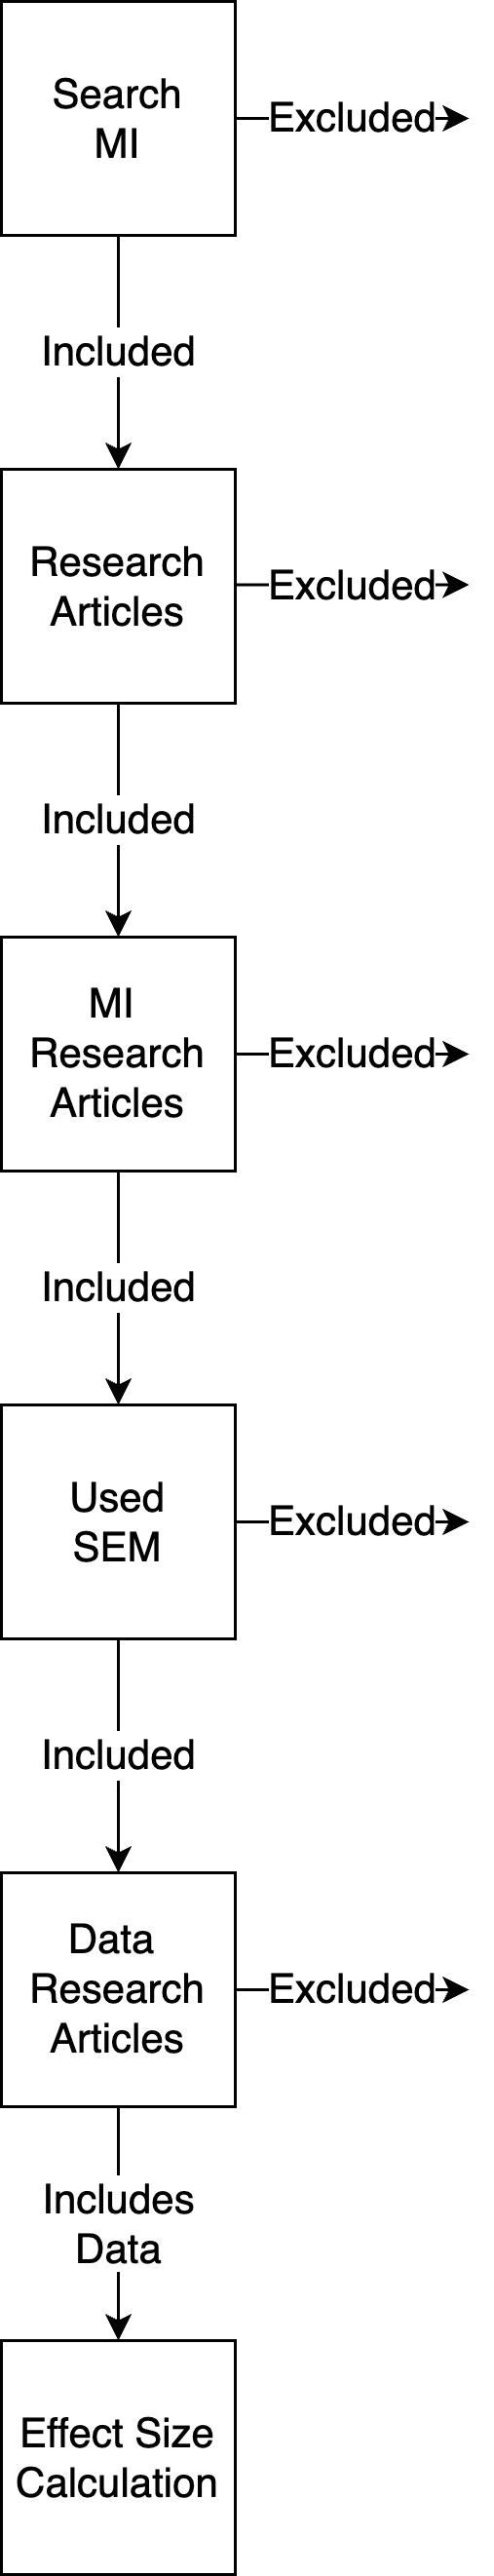
\includegraphics[width=1.69in]{../pics/data_curation} \caption{A flow chart of potential exclusions to create the database of measurement invariance.}\label{fig:figure-process}
\end{figure}

Using \emph{Assessment}'s online search feature, we will search for \textbf{measurement invariance} allowing for either term to be present in the manuscript for inclusion in the first round of papers. As of February 2024, this search returns over 600 articles from 1994 to 2024 publications. The data will then be filtered to only include research articles under the article type filter present on the journal website. These citations will be exported to the Zotero group created for this project found at: \url{https://www.zotero.org/groups/5407184/measurement_invariance_assessment}. Figure \ref{fig:figure-process} displays the filtering and coding process to create the measurement invariance database.

Each article will then be coded for inclusion in the measurement invariance database and for potential further analysis. The coding scale is included in Appendix A. Coders will be first asked to determine if the article includes measurement invariance, and they will be instructed to include articles that use structural equation modeling or item response theory or leave notes if they are unsure. For articles marked yes or unsure, they will then enter if the article uses structural equation modeling or item response theory, as well as a potential other category. Last, they will indicate if the article includes real data. At this point in the survey, studies that have been marked as not measurement variance, item response theory, or simulation/theoretical articles will be excluded.

The next portion of the coding survey includes information about the measurement invariance test(s) in the manuscript. Each measurement test will be coded separately. Coders will include the name and citation of the scale assessed, what groups are compared in the measurement invariance test, and the steps performed in the measurement invariance assessment. Once these steps are selected, coders will order them based on the manuscript, list the type of invariance claimed, and list the fit index used for determination of invariance, along with the rule (i.e., CFI, \(\Delta\)CFI \textgreater{} .01). Finally, they will determine if the data (covariance/correlation matrices or raw data) is avaliable. If so, they will upload it to a private repository for the analysis portion of the study. Coders will be recruited from author networks specifically for individuals with experience in structural equation modeling. They will be given a video example of the coding procedure to watch before beginning the process.

A pilot test of this coding procedure was completed with the lead author's structural equation modeling course. Each coder was assigned a specific issue of Volume 30 and examined all articles within that issue. Approximately 38.30 percent of articles within those issues included measurement invariance (\emph{n} = 120 unique articles coded). Of those articles, 66.70 \% used structural equation modeling, and of those articles, 89.20 percent used participant data. 45 measurement invariance tests were coded, and approximately 42.20 percent included data for testing.

If the search results online return articles that are more closely aligned with measurement invariance (rather than examining all articles as we did in the pilot study), we might expect that a smaller proportion will be excluded for only discussing measurement invariance. If the other percentages are approximate, then we might expect that 400 articles would use structural equation modeling, 357 would include participant data, and 151 may have avaliable data for examination. Given the recent trends in transparency and openness, this number is likely an overestimate as the pilot included only new articles.

The final coding of articles and their measurement invariance tests will be presented as a database of measurement invariance results. These results can be re-used in other meta-analytic studies. We will present the following summary statistics:

\begin{itemize}
\tightlist
\item
  Prevalence of Measurement Invariance

  \begin{itemize}
  \tightlist
  \item
    Total number of invariance related articles
  \item
    Split of articles into structural equation modeling, item response theory, and other analyses types
  \item
    Number of articles that include participant data
  \end{itemize}
\end{itemize}

Each of these statistics will be calculated on the unique articles coded.

\begin{itemize}
\tightlist
\item
  Measurement Invariance Test Statistics

  \begin{itemize}
  \tightlist
  \item
    Commonly reported scales (if any patterns emerge)
  \item
    Frequency of number of groups compared
  \item
    Commonly occurring group comparisons: we will code this variable into overall category such as age, gender/sex, language, etc.
  \item
    Frequency of each type of measurement invariance assessment (i.e., number of equal form, equal item intercepts, etc.)
  \item
    Commonly used fit statistics and rules of thumb for invariance testing
  \item
    Commonly reported level of invariance
  \item
    Frequency of data inclusion for reproducibility
  \end{itemize}
\end{itemize}

\hypertarget{data-analysis}{%
\subsection{Data Analysis}\label{data-analysis}}

Each measurement invariance test that included data will then be coded using the template in Appendix 2. Using the \texttt{visualizemi} package {[}CITE{]}, coders will program a multigroup confirmatory factor analysis using the steps outlined from the research article and the provided data. Each model will first be examined for convergence across the same measurement invariance steps from the published articles. Models that do not converge will be noted, and no more coding will be performed. Given the results from the article, each model will then be tested for replication effect sizes rates at the model and parameter level. For example, an article that claimed measurement invariance for equal form, loadings, and intercepts will be tested with these same steps to determine the effect size of potential replication for each of those steps.

The \texttt{visualizemi} package calculates the effect size of potential replication by bootstrapping the original data with replacement from the study and compares these results to a the same bootstrapped dataset that has had the group labels randomized. The effect size is normalized based on the range of \emph{h} (effect size for two proportions, similar to Cohen's \emph{d}) to create a score of -1 to 1. A positive non-measurement invariance effect size means that the bootstrapped data has more non-invariance than the randomized scores. A negative effect size would indicate that the bootstrapped data has less non-invariance than the randomized data. A score of zero indicates that the bootstrapped and randomized data have the same likelihood of (non)-invariance. The logic of desiring a zero or negative effect size is that it implies that the groups are equivalent, and therefore, the randomization does not affect the results because groups perform the same on the questionnaire. Because this effect size is based on proportions, one could flip the sign for the effect size for measurement invariance, but here we focus on the amount of non-invariance.

The potential ``partial'' invariance for each parameter at the final step of the model testing will then be examined. In our example, the intercept level would be examined for parameter level effect sizes, as it was the final step of their invariant model. If an article reported partial invariance, the step with partial invariance will be examined at the parameter level. If they used multiple partial invariance steps, only the final stage will be examined. The same effect size can be calculated for each parameter in the partial invariance test, as well as the difference in group parameter estimates (i.e., \emph{d} for intercept group 1 versus intercept group 2).

Each coding will be programmed by one coder and checked by another coder using a small number of bootstrap simulations. After both agree that the coding matches the article data, the model and parameter level simulations will be run over 1000 simulations on a high performance computing server to ensure consistency in versions of \emph{R} and packages. The exact versions will be reported for reproducibility. The results will be exported in both an HTML format and Rdata for further use. These files will be available on our repository at \url{https://github.com/doomlab/assessment-squared}.

\hypertarget{model-level-results}{%
\subsubsection{Model Level Results}\label{model-level-results}}

At the model level, the bootstrapping function returns an effect size \texttt{h\_nmi\_p} which represents the \emph{h} effect size statistic for measurement invariance normalized to a proportion of the possible effect size ranged. We will compile the results based on step across measurement invariance tests, and we will report the following (simulated data below):

\begin{itemize}
\tightlist
\item
  Mean, standard deviation, sample size for each step
\item
  25, 50, 75\% quantile values
\item
  Visualization of the distribution of effects - for example, Figure \ref{fig:figure-violin}
\end{itemize}

\begin{figure}
\centering
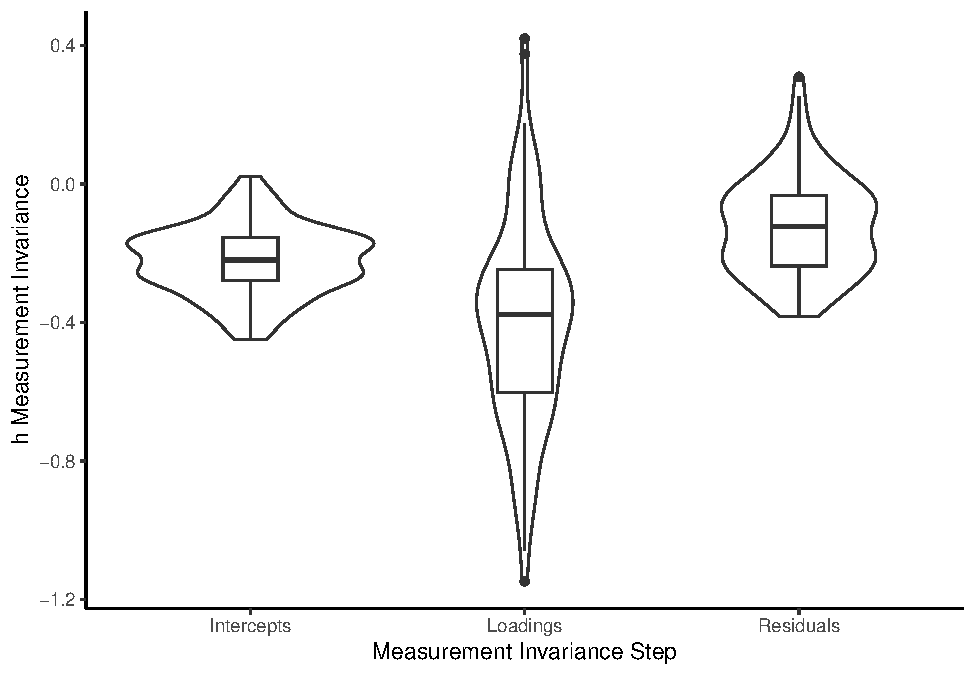
\includegraphics{rr_manuscript_files/figure-latex/figure-violin-1.pdf}
\caption{\label{fig:figure-violin}A visualization of the effect sizes for measurement invariance at the model level.}
\end{figure}

\hypertarget{parameter-level-results}{%
\subsubsection{Parameter Level Results}\label{parameter-level-results}}

For the parameter level results, the bootstrapping function returns similar information for each of the parameters in the final step of the model. For example, if a manuscript suggests that the model was fully invariant at the residuals level, each residual effect would be tested to determine effect sizes of replication and group differences. First, we will extract the \texttt{h\_nmi\_p} effects for each parameter to determine the distribution, statistics, and visualizations for each type of parameter (loadings, residuals, intercepts, etc.). We will present:

\begin{itemize}
\tightlist
\item
  Mean, standard deviation, sample size for each type of parameter
\item
  25, 50, 75\% quantile values
\item
  Visualization of the distribution of effects
\end{itemize}

Next, the function additionally returns effect sizes for group differences on each parameter, \(d_s\). This value is calculated as the average mean difference of the parameter estimates for each group divided by their pooled standard error across bootstraps. \(d_s\) is calculated for both the bootstrapped data and the randomized data. We will calculated a ``normalized'' effect size for each parameter by subtracting \(d_s\) for the bootstrapped data minus the \(d_s\) for the randomized data. Because group order is arbitrary in our analysis, we will take the absolute value of the effect size for final reporting. From this dataset, we will report:

\begin{itemize}
\tightlist
\item
  Mean, standard deviation, sample size for each type of parameter
\item
  25, 50, 75\% quantile values
\item
  Visualization of the distribution of effects
\end{itemize}

\hypertarget{results-interpretation}{%
\subsection{Results Interpretation}\label{results-interpretation}}

Our study is exploratory to determine the landscape of measurement invariance effect size using the premier journal outlet for such publications in clinical psychology. We make no predictions on the direction or size of the results. Instead, we will present the database for future reuse and examine the results for any consistent patterns or findings. By understanding the range of published values\footnote{The advantage of studying measurement invariance in this scenario is that both invariant and non-invariant models are typically publishable. While publication bias likely still exists, it may be less than traditional effect size meta-analysis studies.}, researchers can use these results to gauge their study results against. We will comment on potential ideas for estimating the smallest effect of interest for measurement invariance.

\newpage

\hypertarget{references}{%
\section{References}\label{references}}

\hypertarget{refs}{}
\begin{CSLReferences}{1}{0}
\leavevmode\vadjust pre{\hypertarget{ref-anvari2021}{}}%
Anvari, F., \& Lakens, D. (2021). Using anchor-based methods to determine the smallest effect size of interest. \emph{Journal of Experimental Social Psychology}, \emph{96}, 104159. \url{https://doi.org/10.1016/j.jesp.2021.104159}

\leavevmode\vadjust pre{\hypertarget{ref-barry2014}{}}%
Barry, A. E., Chaney, B., Piazza-Gardner, A. K., \& Chavarria, E. A. (2014). Validity and Reliability Reporting Practices in the Field of Health Education and Behavior: A Review of Seven Journals. \emph{Health Education \& Behavior}, \emph{41}(1), 12--18. \url{https://doi.org/10.1177/1090198113483139}

\leavevmode\vadjust pre{\hypertarget{ref-byrne2001}{}}%
Byrne, B. M. (2001). Structural Equation Modeling With AMOS, EQS, and LISREL: Comparative Approaches to Testing for the Factorial Validity of a Measuring Instrument. \emph{International Journal of Testing}, \emph{1}(1), 55--86. \url{https://doi.org/10.1207/S15327574IJT0101_4}

\leavevmode\vadjust pre{\hypertarget{ref-byrne1989}{}}%
Byrne, B. M., Shavelson, R. J., \& Muthén, B. (1989). Testing for the equivalence of factor covariance and mean structures: The issue of partial measurement invariance. \emph{Psychological Bulletin}, \emph{105}(3), 456--466. \url{https://doi.org/10.1037/0033-2909.105.3.456}

\leavevmode\vadjust pre{\hypertarget{ref-cheung2000}{}}%
Cheung, G. W., \& Rensvold, R. B. (2000). Assessing Extreme and Acquiescence Response Sets in Cross-Cultural Research Using Structural Equations Modeling. \emph{Journal of Cross-Cultural Psychology}, \emph{31}(2), 187--212. \url{https://doi.org/10.1177/0022022100031002003}

\leavevmode\vadjust pre{\hypertarget{ref-devellis2022}{}}%
DeVellis, R. F., \& Thorpe, C. T. (2022). \emph{Scale development: Theory and applications} (Fifth edition). SAGE Publications, Inc.

\leavevmode\vadjust pre{\hypertarget{ref-dong2020}{}}%
Dong, Y., \& Dumas, D. (2020). Are personality measures valid for different populations? A systematic review of measurement invariance across cultures, gender, and age. \emph{Personality and Individual Differences}, \emph{160}, 109956. \url{https://doi.org/10.1016/j.paid.2020.109956}

\leavevmode\vadjust pre{\hypertarget{ref-flake2020}{}}%
Flake, J. K., \& Fried, E. I. (2020). Measurement schmeasurement: Questionable measurement practices and how to avoid them. \emph{Advances in Methods and Practices in Psychological Science}, \emph{3}(4), 456465. \url{https://doi.org/10.1177/2515245920952393}

\leavevmode\vadjust pre{\hypertarget{ref-lakens2018}{}}%
Lakens, D., Scheel, A. M., \& Isager, P. M. (2018). Equivalence Testing for Psychological Research: A Tutorial. \emph{Advances in Methods and Practices in Psychological Science}, \emph{1}(2), 259--269. \url{https://doi.org/10.1177/2515245918770963}

\leavevmode\vadjust pre{\hypertarget{ref-liu2017}{}}%
Liu, M., Harbaugh, A. G., Harring, J. R., \& Hancock, G. R. (2017). The effect of extreme response and non-extreme response styles on testing measurement invariance. \emph{Frontiers in Psychology}, \emph{8}, 726. \url{https://doi.org/10.3389/fpsyg.2017.00726}

\leavevmode\vadjust pre{\hypertarget{ref-maassen2023}{}}%
Maassen, E., D'Urso, E. D., Van Assen, M. A. L. M., Nuijten, M. B., De Roover, K., \& Wicherts, J. M. (2023). The dire disregard of measurement invariance testing in psychological science. \emph{Psychological Methods}. \url{https://doi.org/10.1037/met0000624}

\leavevmode\vadjust pre{\hypertarget{ref-marsh2004}{}}%
Marsh, H. W., Hau, K.-T., \& Wen, Z. (2004). In search of golden rules: Comment on hypothesis-testing approaches to setting cutoff values for fit indexes and dangers in overgeneralizing hu and bentler's (1999) findings. \emph{Structural Equation Modeling: A Multidisciplinary Journal}, \emph{11}(3), 320--341. \url{https://doi.org/10.1207/s15328007sem1103_2}

\leavevmode\vadjust pre{\hypertarget{ref-meredith1993}{}}%
Meredith, W. (1993). Measurement invariance, factor analysis and factorial invariance. \emph{Psychometrika}, \emph{58}(4), 525--543. \url{https://doi.org/10.1007/BF02294825}

\leavevmode\vadjust pre{\hypertarget{ref-nye2011}{}}%
Nye, C. D., \& Drasgow, F. (2011). Effect size indices for analyses of measurement equivalence: Understanding the practical importance of differences between groups. \emph{Journal of Applied Psychology}, \emph{96}(5), 966--980. \url{https://doi.org/10.1037/a0022955}

\leavevmode\vadjust pre{\hypertarget{ref-putnick2016}{}}%
Putnick, D. L., \& Bornstein, M. H. (2016). Measurement invariance conventions and reporting: The state of the art and future directions for psychological research. \emph{Developmental Review}, \emph{41}, 71--90. \url{https://doi.org/10.1016/j.dr.2016.06.004}

\leavevmode\vadjust pre{\hypertarget{ref-vandeschoot2015}{}}%
Van De Schoot, R., Schmidt, P., De Beuckelaer, A., Lek, K., \& Zondervan-Zwijnenburg, M. (2015). Editorial: Measurement invariance. \emph{Frontiers in Psychology}, \emph{6}. \url{https://www.frontiersin.org/articles/10.3389/fpsyg.2015.01064}

\leavevmode\vadjust pre{\hypertarget{ref-weidman2017}{}}%
Weidman, A. C., Steckler, C. M., \& Tracy, J. L. (2017). The jingle and jangle of emotion assessment: Imprecise measurement, casual scale usage, and conceptual fuzziness in emotion research. \emph{Emotion}, \emph{17}(2), 267--295. \url{https://doi.org/10.1037/emo0000226}

\leavevmode\vadjust pre{\hypertarget{ref-wicherts2005}{}}%
Wicherts, J. M., Dolan, C. V., \& Hessen, D. J. (2005). Stereotype Threat and Group Differences in Test Performance: A Question of Measurement Invariance. \emph{Journal of Personality and Social Psychology}, \emph{89}(5), 696--716. \url{https://doi.org/10.1037/0022-3514.89.5.696}

\end{CSLReferences}

\newpage

\hypertarget{appendix-appendix}{%
\appendix}


\hypertarget{inclusion-survey}{%
\section{Inclusion Survey}\label{inclusion-survey}}

You will use this form to code articles for the Measurement Invariance Project. You should fill out this form once for each article. If the article has multiple measurement invariance tests (i.e., once for sex and once for age), then you would fill out the article once for for each test of measurement invariance within an article.

Note: the survey will end if your article does not have the required components we are looking for in the article. If you think you did something wrong, please ask or simply recode it.

\hypertarget{page-1}{%
\subsection{Page 1}\label{page-1}}

Enter the article doi as an html link (i.e., \url{https://doi.org/10.1177/107319119400100401}):

\hypertarget{page-2}{%
\subsection{Page 2}\label{page-2}}

Does this article report measurement invariance?

Search the document (control + F) for equal groups, invariance, multigroup. Notes:

\begin{itemize}
\tightlist
\item
  Code yes even if the data is simulated
\item
  Code yes if item response theory differential item functioning is used
\item
  Code other for unsure or unclear or list your own reason
\end{itemize}

Options: Yes, No, Other

\emph{Survey will end if No is selected}

\hypertarget{page-3}{%
\subsection{Page 3}\label{page-3}}

Does this article use structural equation modeling (confirmatory factor analysis) or item response theory?

Options: Structural Equation Modeling, Item Response Theory, Neither: List Analysis

\emph{Survey will end if IRT is selected}

\hypertarget{page-4}{%
\subsection{Page 4}\label{page-4}}

Does this article include real data (i.e., no simulation studies)?

Options: Yes, No, Unclear

\emph{Survey will end if No is selected}

\hypertarget{page-5}{%
\subsection{Page 5}\label{page-5}}

What is the name of the instrument/scale they are testing? Please include the entire name, not the abbreviation.

What is the citation of the scale they are testing? Copy from the reference section.

\hypertarget{page-6}{%
\subsection{Page 6}\label{page-6}}

How many groups are compared?

What sample groups are they comparing in this analysis? List groups the way they are described (i.e., do not correct Male/Female to Men/Women, use the names from the paper). Separate groups with a comma.

\hypertarget{page-7}{%
\subsection{Page 7}\label{page-7}}

What steps of measurement invariance did they test? Please click all that were used. The names in parentheses are sometimes used to describe each step.

Multiple Option Select: Equal form (configural), equal item loadings (metric), equal item intercepts/means (scalar), equal item thresholds, equal item residuals (strict), equal item residual covariances, equal latent means (population means), equal latent variances, equal latent covariances, equal regressions

\hypertarget{page-8}{%
\subsection{Page 8}\label{page-8}}

What order did they test the steps in? Please drag and drop them into the order found in the paper (often in a table).

Options are piped in from previous question.

\hypertarget{page-9}{%
\subsection{Page 9}\label{page-9}}

What metric did they use to assess measurement invariance? (i.e., CFI, RMSEA, other fit measures, you can use abbreviations of fit indices)

What rule did they use for measurement invariance? (i.e., change in CFI \textless{} .01, chi-square difference test, etc.). List the rule as what would be considered invariant (i.e., passes the test, groups are considered equal).

What type of invariance did they claim? Use the step name and their words for the type of invariance. For example, fully invariant to residuals/strict, partially scalar invariant, non-invariant, etc.)

\hypertarget{page-10}{%
\subsection{Page 10}\label{page-10}}

Is the data accessible? Look for supplemental documents, links to files, and pages of correlation/covariance matrices.

Options: Matrices included, contact author, No, Unclear or Broken Links

\hypertarget{page-11}{%
\subsection{Page 11}\label{page-11}}

If the data is available, researchers will be given instructions on how to download it for the next stage of the project, to be shared with analysts.

\hypertarget{example-data-analysis-code}{%
\section{Example Data Analysis Code}\label{example-data-analysis-code}}

\hypertarget{libraries}{%
\subsection{Libraries}\label{libraries}}

\hypertarget{data}{%
\subsection{Data}\label{data}}

\hypertarget{model-programming}{%
\subsection{Model Programming}\label{model-programming}}

Program the model in \texttt{lavaan} syntax including all correlated errors or other adjustments noted by the original authors.

\hypertarget{use-mgcfa-function}{%
\subsection{Use MGCFA function}\label{use-mgcfa-function}}

Use the \texttt{mgcfa} function to run the proposed model steps. This model should replicate their model excluding any partial invariance steps. If they say they will run ``residuals'' but then do not because of partial invariance, only include up to the step that was invariant or partially invariant.

\hypertarget{review-model-outputs}{%
\subsection{Review Model Outputs}\label{review-model-outputs}}

Review model outputs to ensure they do not produce heywood cases or other errors.

\begin{verbatim}
## # A tibble: 7 x 18
##    agfi   AIC   BIC   cfi chisq  npar  rmsea rmsea.conf.high   srmr   tli
##   <dbl> <dbl> <dbl> <dbl> <dbl> <dbl>  <dbl>           <dbl>  <dbl> <dbl>
## 1 0.991 7535. 7647. 0.931  85.3    30 0.0921           0.114 0.0595 0.896
## 2 0.989 3671. 3761. 0.906  61.4    30 0.103            0.136 0.0749 0.859
## 3 0.991 3846. 3938. 0.959  44.4    30 0.0741           0.108 0.0525 0.938
## 4 0.990 7518. 7740. 0.935 106.     60 0.0894           0.113 0.0634 0.903
## 5 0.989 7526. 7726. 0.919 126.     54 0.0943           0.116 0.0741 0.892
## 6 0.989 7533. 7711. 0.905 145.     48 0.0970           0.117 0.0753 0.886
## 7 0.988 7537. 7682. 0.890 167.     39 0.0972           0.116 0.0926 0.886
## # i 8 more variables: converged <lgl>, estimator <chr>, ngroups <int>,
## #   missing_method <chr>, nobs <int>, norig <int>, nexcluded <int>, model <chr>
\end{verbatim}

\begin{verbatim}
## lavaan 0.6.17 ended normally after 35 iterations
## 
##   Estimator                                         ML
##   Optimization method                           NLMINB
##   Number of model parameters                        30
## 
##   Number of observations                           301
## 
## Model Test User Model:
##                                                       
##   Test statistic                                85.306
##   Degrees of freedom                                24
##   P-value (Chi-square)                           0.000
\end{verbatim}

\hypertarget{replication-model-level}{%
\subsection{Replication Model Level}\label{replication-model-level}}

Run the \texttt{bootstrap\_model} function and determine the effect sizes for model level invariance steps. Use the same \texttt{group.equal} constraints as above.

\begin{verbatim}
## Finished Bootstrap Number: 1
## Finished Bootstrap Number: 2
## Finished Bootstrap Number: 3
## Finished Bootstrap Number: 4
## Finished Bootstrap Number: 5
## Finished Bootstrap Number: 6
## Finished Bootstrap Number: 7
## Finished Bootstrap Number: 8
## Finished Bootstrap Number: 9
## Finished Bootstrap Number: 10
## Finished Bootstrap Number: 11
## Finished Bootstrap Number: 12
## Finished Bootstrap Number: 13
## Finished Bootstrap Number: 14
## Finished Bootstrap Number: 15
## Finished Bootstrap Number: 16
## Finished Bootstrap Number: 17
## Finished Bootstrap Number: 18
## Finished Bootstrap Number: 19
## Finished Bootstrap Number: 20
\end{verbatim}

\begin{tabular}{l|r|r|r|r|r|r}
\hline
model & non\_invariant & random\_non\_invariant & h\_nmi & h\_mi & h\_nmi\_p & h\_mi\_p\\
\hline
intercepts & 0.20 & 0.0 & 0.9272952 & -0.9272952 & 0.2951672 & -0.2951672\\
\hline
loadings & 0.75 & 0.1 & 1.4508940 & -1.4508940 & 0.4618339 & -0.4618339\\
\hline
residuals & 0.05 & 0.0 & 0.4510268 & -0.4510268 & 0.1435663 & -0.1435663\\
\hline
\end{tabular}

\hypertarget{replication-parameter-level-partial-invariance}{%
\subsection{Replication Parameter Level / Partial Invariance}\label{replication-parameter-level-partial-invariance}}

If their model was invariant: use the last step as the \texttt{partial\_step} option. If their model was partially invariant, use the step that was indicated as partially invariant (where they had to relax parameters - if they did this on more than one step, use the last one).


\end{document}
